%template1.tex
%The following LaTeX source file represents the simplest kind of slide presentation; no overlays, no included graphics. Substitute your favorite style for ``pascal''. To create the PDF file template1.pdf, (1) be sure to use the prosper class, then (2) execute the command latex template1.tex, and (3) the command dvipdf template1.dvi.

%%%%%%%%%%%%%%%%%%%%%%%%%%%%%%% template1.tex %%%%%%%%%%%%%%%%%%%%%%%%%%%%%%%%%%%
\documentclass[a4paper,blends,pdf,colorBG,slideColor]{prosper}
% definitions for slides for CSC544
% Lutz Hamel, (c) 2007

\hypersetup{pdfpagemode=FullScreen}

\usepackage{amssymb}
\usepackage{latexsym}
\usepackage{amsmath}
%\usepackage[usenames]{color}
\usepackage{xypic}


\newcommand{\term}[1]{\ensuremath{\mbox{\bf #1}}}
\newcommand{\nonterm}[1]{\ensuremath{\mbox{#1}}}
\newcommand{\ifstmt}[3]{\ensuremath{{\bf if}\; {#1}\;{\bf then}\;{#2}\;{\bf else}\;{#3}\;\term{end}}}
\newcommand{\whilestmt}[2]{\ensuremath{{\bf while}\; {#1}\;{\bf do}\;{#2}\; \term{end}}}
\newcommand{\funcstmt}[3]{\ensuremath{{\bf fun}\; {#1}\; {\bf is}\; {#2} \; {\bf return}\; {#3}}}
\newcommand{\syntaxset}[1]{\ensuremath{\mbox{\bf #1}}}
\newcommand{\orbar}{\;|\;}
\newcommand{\bs}[1]{\begin{slide}{#1}\ptsize{8}}
\newcommand{\es}{\end{slide}}
\newcommand{\co}{\,\colon\;}
\newcommand{\pair}[2]{\ensuremath{\langle {#1}, {#2} \rangle}}
\newcommand{\encode}[1]{\ensuremath{\langle {#1} \rangle}}
\newcommand{\mytab}{\makebox[.15in]{}}
%\newcommand{\abs}[1]{{\mid{#1}\mid}}
\newcommand{\abs}[1]{{|{#1}|}}
\newcommand{\ol}[1]{\overline{#1}}

\newcommand{\qaccept}{\ensuremath{q_{\mbox{\tiny accept}}}}
\newcommand{\qreject}{\ensuremath{q_{\mbox{\tiny reject}}}}
\newcommand{\accept}{{\em accept}}
\newcommand{\reject}{{\em reject}}

\newcommand{\machine}[1]{
	\begin{quote}
	{#1}
	\end{quote}
	}

\newcommand{\fdef}[1]{
	\begin{center}
	\fbox{
	\begin{minipage}{3.5in}
	{\bf Definition:}
	{#1}
	\end{minipage}
	}
	\end{center}
	}

\newcommand{\ftheorem}[1]{
	\begin{center}
	\fbox{
	\begin{minipage}{3.5in}
	{\bf Theorem:}
	{#1}
	\end{minipage}
	}
	\end{center}
	}

\newcommand{\flemma}[1]{
	\begin{center}
	\fbox{
	\begin{minipage}{3.5in}
	{\bf Lemma:}
	{#1}
	\end{minipage}
	}
	\end{center}
	}


\newcommand{\fframe}[1]{
	\begin{center}
	\fbox{
	\begin{minipage}{3.5in}
	{#1}
	\end{minipage}
	}
	\end{center}
	}

\newcommand{\nframe}[1]{
	\begin{center}
	\begin{minipage}{3.5in}
	{#1}
	\end{minipage}
	\end{center}
	}

\begin{document}

\bs{Alternate Definition}
\vspace{.2in}
\fdef{
A {\bf\em Turing-recognizable language} is a formal language for which there exists a Turing machine that will halt and accept when presented with any string in the language as input but may either halt and reject or loop forever when presented with a string not in the language. Contrast this to {\bf\em (Turing-)decidable languages}, which require that the Turing machine halts in all cases.
}
\vspace{.5in}
{\small Source: Wikipedia}

\es

\bs{Decidable Languages}
\begin{center}
\includegraphics[height=60mm]{images/tm-example_0001.eps}
\end{center}
\es

\bs{Decidable Languages}
\begin{center}
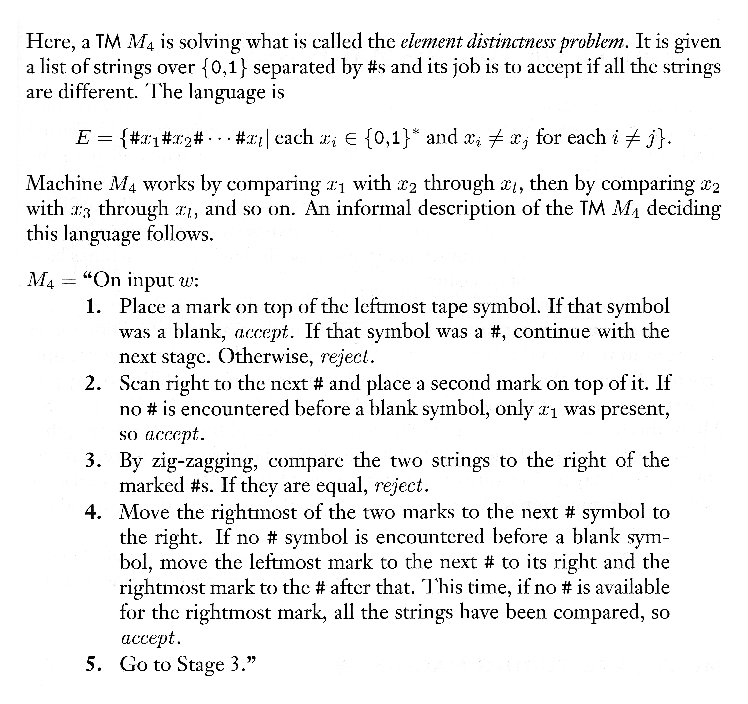
\includegraphics[height=70mm]{images/tm-example_0002.eps}
\end{center}
\es

\bs{Variants of TM's}
As in the case of FA's we can construct different variants of the Turing machine. And, as
in the case of FA's, we can show that all these variants have the same computational 
power: they all recognize the same languages.\footnote{This is not to be confused with 
{\em complexity}, some of the variants have lower computational complexity than others 
for the same task.}

The most important variants:
\begin{itemize}
\item multi-tape TM's
\item nondeterministic TM's
\end{itemize}

\vspace{1in}
\es

\bs{Multi-tape TM's}
{\scriptsize
\fframe{
A {\bf\em multi-tape Turing machine} is a $7$-tuple, 
$
(Q,\Sigma,\Gamma,\delta,q_0,\qaccept,\qreject),
$
where $Q,\Sigma,\Gamma$ are  all finite sets and
\begin{enumerate}
\item $Q$ is the set of states,
\item $\Sigma$ is the input alphabet not containing the {\bf\em blank symbol} $\sqcup$,
\item $\Gamma$ is the tape alphabet, where $\sqcup \in \Gamma$ and $\Sigma \subseteq \Gamma$,
\item $\delta\co Q \times \Gamma^k \rightarrow Q\times\Gamma^k\times\{L,R\}^k$ is
the transition function with $k$ the number of tapes,
\item $q_0\in Q$ is the start state,
\item $\qaccept\in Q$ is the accept state, and
\item $\qreject\in Q$ is the reject state, where $\qreject \ne \qaccept$.
\end{enumerate}
}
}
\begin{center}
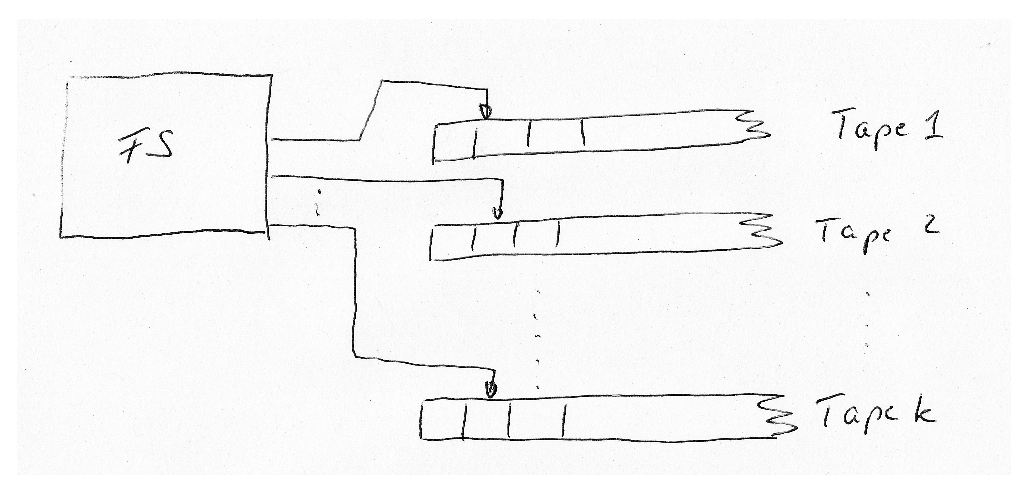
\includegraphics[height=20mm]{images/mt-tm.eps}
\end{center}
{\bf NOTE:} For convenience sake we always load the input onto tape 1.
\es

\bs{Multi-tape TM's}
\fframe{{\bf Theorem:} Multi- and Single-tape TM's are equivalent.}

{\bf Proof Sketch:} We show equivalence by demonstrating that each machine can 
simulate the other.

(a) To show that a multi-tape TM can simulate a single-tape TM is trivial because a
single-tape TM is a special case of the multi-tape TM.

(b) A single-tape TM can simulate a multi-tape TM by simulating the $k$ tapes of the
multi-tape machine on its single tape.  This requires appropriate separation markers between the virtual tapes and
memory for the $k$ virtual tape heads.  Graphically,
\begin{center}
\includegraphics[height=25mm]{images/mt-tm-example.eps}
\end{center}
$\Box$
\es

\bs{Multi-tape TM's}
\vspace{.5in}
\fframe{{\bf Corollary:} A language is Turing-recognizable iff some multi-tape TM
recognizes it.}
\es

\bs{Nondeterministic TM's}
{\scriptsize
\fframe{
A {\bf\em nondeterministic Turing machine} is a $7$-tuple, 
$
(Q,\Sigma,\Gamma,\delta,q_0,\qaccept,\qreject),
$
where $Q,\Sigma,\Gamma$ are  all finite sets and
\begin{enumerate}
\item $Q$ is the set of states,
\item $\Sigma$ is the input alphabet not containing the {\bf\em blank symbol} $\sqcup$,
\item $\Gamma$ is the tape alphabet, where $\sqcup \in \Gamma$ and $\Sigma \subseteq \Gamma$,
\item $\delta\co Q \times \Gamma \rightarrow {\color{red}P(Q\times\Gamma\times\{L,R\})}$ is
the transition function,
\item $q_0\in Q$ is the start state,
\item $\qaccept\in Q$ is the accept state, and
\item $\qreject\in Q$ is the reject state, where $\qreject \ne \qaccept$.
\end{enumerate}
}
}
\begin{minipage}{2in}
\includegraphics[height=35mm]{images/ntm-computation.eps}
\end{minipage}
\begin{minipage}{2in}
{\bf NOTE:} If all branches of computation in an NTM halt on 
all inputs then we call it a {\bf\em decider}.
\end{minipage}

\es

\bs{Nondeterministic TM's}
\fframe{{\bf Theorem:} Nondeterministic TM's are equivalent to deterministic TM's.}

{\bf Proof Sketch:} We show equivalence by showing that each TM can simulate the other.

(a) To show that nondeterministic TM's can simulate deterministic TM's is trivial because
deterministic TM's are a special case of nondeterministic TM's.

(b) We can simulate an NTM $N$ with a TM $D$ by having $D$ search through the
tree of nondeterministic computation configurations for accepting configurations
in a {\em breadth first} manner.
$\Box$

\fframe{{\bf Corollary:} A language is Turing-recognizable iff some nondeterministic TM recognizes it}

\fframe{{\bf Corollary:} A language is decidable iff some nondeterministic TM decides it}

\es

\bs{Encodings}
Since TM's are models of general computations we are able to express  algorithms
over more structured problems than just structures of strings.

We express more general encodings as \encode{\mbox{something}}.
The thing to keep in mind is that this encoding should be ``straight forward'' in the
sense that the process of encoding should not hide steps that might lead
to erroneous conclusions when computing with TM's.\footnote{This will become especially important when we talk about computational complexity.}

{\bf Example:} Let $A$ be the language of all connected undirected graphs, formally
\[
A = \{ \encode{G} | \mbox{$G$  is a connected undirected graph}\}.
\]
We could envision that \encode{G} is a list of vertices and the edges between them
easily obtained by scanning the graph $G$.
\vspace{.2in}
\es

\bs{Encodings}
{\bf Example:} Show that the language
\[
A = \{ \encode{G} | \mbox{$G$  is a connected undirected graph}\}.
\]
is decidable.

{\bf Proof:} We show decidability by constructing a decider for the language.
\begin{center}
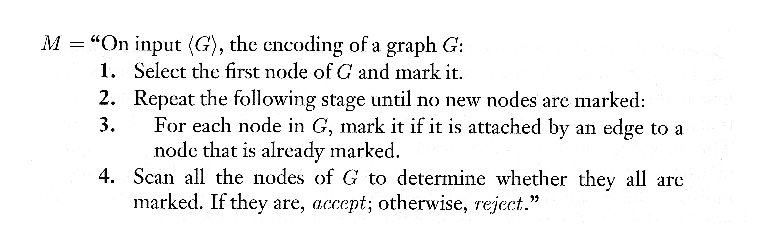
\includegraphics[height=25mm]{images/graph-decider.eps}
\end{center}

\es
\end{document}
%%%%%%%%%%%%%%%%%%%%%%%%%%% end of template1.tex %%%%%%%%%%%%%%%%%%%%%%%%%%%%%%%%

